

\chapter{Ασύρματα Επαναφορτιζόμενα Δίκτυα Αισθητήρων}\label{ch:wrsns}
\section{Η Ιστορία Πίσω Από την Τεχνολογία}
Οι προσπάθειες ασύρματης μεταφοράς ενέργειας πρωτοσυναντόνται πίσω στα τέλη του 19ου αιώνα, πολύ πριν την εγκατάσταση ενσύρματης μεταφοράς ενέργειας. Ο Νικόλα Τέσλα
από το 1891 είχε καταφέρει να μεταφέρει ενέργεια ασύρματα μέσα από επαγωγή μεγάλων πηνείων. Η εφεύρεση αυτή τον είχε εντυπωσιάσει τόσο πολύ όσο τίποτα άλλο που
μάλιστα δήλωσε οτι αυτή η εφεύρεσή του θα ήταν η πιο πολύτιμη από όλες. Tο 1899, ο Νικολά Τέσλα, μεταφέρθηκε στα εργαστήρια της εταιρείας Colorado Springs όπου
εμβάθυνε ακόμα περισσότερο στην τεχνολογία αυτή. Το 1902 κατέθεσε μια πατέντα \cite{tesla_patent} για μία συσκευή η οποία ήταν προιόν αυτής της έρευνας. Ήταν ένα
πηνίο σε διάταξη Τέσλα το οποίο μετέφερε ενέργεια χρησιμοποιώντας μεταφορά ενέργειας σε ιδιοσυχνότητα από το κάτω πηνίο σε μερικά μέτρα στο πάνω πηνίο. Αυτό
επιτρέπει να δημιουργηθούν πολύ υψηλές τάσεις και διάταξη (Πηνία Τέσλα - Tesla Coils) που χρησιμοποιείται στην πράξη και σήμερα.

\begin{figure}[h]
  \centering
  \subfloat{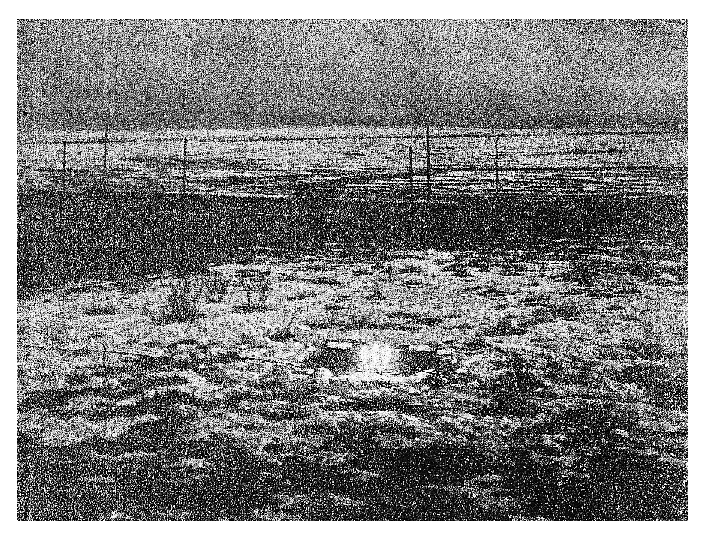
\includegraphics[width=0.62\textwidth]{images/tesla_exper1.eps}}
  \subfloat{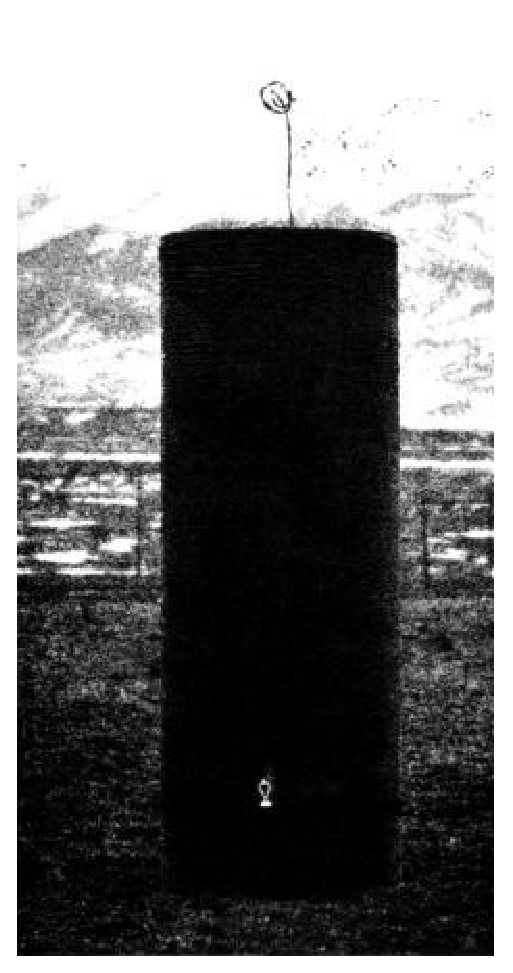
\includegraphics[width=0.32\textwidth]{images/tesla_exper2.eps}}
  \caption{Επιτυχημένες προσπάθειες του Νικόλα Τέσλα μεταφοράς ασύρματης ενέργειας είχαν γίνει από τα τέλη του 19ου αιώνα.}
  \label{fig:tesla_eperiments}
\end{figure}

Εκείνη την εποχή ήταν η ανατολή για την θέσπιση ηλεκτρικής ενέργειας στις συσκευές. Επίσης εκείνη την εποχή μόλις είχε τελειώσει ο πόλεμος των ρευμάτων (the war of
currents) στον οποίο υπήρχαν διαφωνίες στο αν θα έπρεπε στα ηλεκτρικά δίκτυα που επρόκειτο να δημιουργηθούν να είχαν εναλλασσόμενο ρεύμα (AC) ή συνεχές (DC). Όμως
υπήρχαν επιστήμονες και μηχανικοί που συμφωνούσαν οτι η χρησιμοποιήση καλωδίων για την μεταφορά ενέργειας από κάθε τοποθεσία που αναπαράγοταν σε κάθε τοποθεσία που
θα το χρησιμοποιούσε θα ήταν πολύ ακριβό και όχι πρακτικό. Ο Τέσλα ήταν ένας από τους πιο γνωστούς επιστήμονες της εποχής που υποστήριζε αυτή την άποψη και
προσπαθούσε να βρει τρόπους να μεταφέρει ενέργεια ασύρματα. Το όραμά του ήταν ένας ασύρματος κόσμος στον οποίο η ασύρματη μεταφορά ενέργειας και η ασύρματες
επικοινωνίες θα μπορούσαν να φτάσουν σε όλο τον κόσμο, παραδίδοντας ενέργεια και πληροφορίες σε πλοία τα οποία ταξιδεύουν στη θάλασσα, σε εργοστάσια και γενικά σε
κάθε σπίτι του πλανήτη.

Ο Τέσλα έχοντας πάρει μια χορήγησει US\$150.000, ξεκίνησε να κατασκευάζει τον πύργο Wardenclyffe προκειμένου να κάνει το όραμά του πραγματικότητα. Η κατασκευή είχε
ύψος 56 μέτρα και είχε χτιστεί κοντά στην Νέα Υόρκη ενώ το κτήριο κοντά στον πύργο χρησιμοποιόταν ως εργαστήριο. Για την λειτουργία του όμως ο Tέσλα χρειαζόταν
επιπλέον χρηματοδοτήσεις τις οποίες ζητούσε αλλεπάλληλα από τον John Pierpont Morgan ο οποίος ήταν ο κύριος χορηγός του. Ωστόσο ο J. P. Morgan δεν πείστηκε από τις
ικανότητες του κατασκευάσματος του Τέσλα και έτσι σταμάτησε την χρηματοδότηση με συνέπεια το σχέδιο του Τέσλα να σταματήσει εκεί.

\begin{figure}[h]
	\centering
	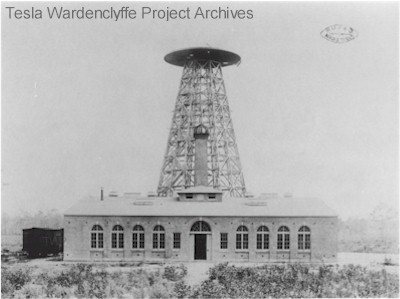
\includegraphics[width=\textwidth]{images/Wardenclyffe_Tower.jpg}
	\caption{Ο πύργος Wardenclyffe ο οποίος χτίστηκε για πειράματα μεταδοσης ασύρματης ενέργεια.}
	\label{fig:Wardenclyffe_Tower}
\end{figure}

Παρόλο που για την εποχή του, ο Τέσλα είχε κατασκευάσει ένα πολύ προηγμένο σύστημα μεταφοράς ενέργειας, είχε πολλά προβλήματα με κύριο τις απώλειες ενέργειας. Καθώς
η συσκευή του Τέσλα εξεπεμπε στον χώρο πολύ δυνατά ηλεκτρομαγνητικά κύματα, προκειμένου να πετύχει μεταφορά ενέργειας σε μεγάλη απόσταση χρειαζόταν τεράστιες
ποσότητες ενέργειας καθώς οι απώλειες ήταν πολύ μεγάλες.

Στις αρχές της δεκαετίας του 1960 η μεταφορά ενέργειας μέσω ιδιοσυχνοτικής ηλεκτρομαγνητικής επαγωγής (resonant inductive coupling) χρησιμοποιήθηκε επιτυχημένα σε
εμφυτεύσιμες συσκευές της ιατρικής όπως βηματοδότες και τεχνητές καρδιές. Τα πρώτα συστήματα είχαν μόνο δέκτη ιδιοσυχνοτικού πηνίου αλλά τα επόμενα συστήματα
ενσωμάτωσαν και πομό ιδιοσυχνοτικού πομπού. Οι συσκευές αυτές είχαν σχεδιαστεί έτσι ώστε να έχουν πολύ μεγάλη απόδοση χρησιμοποιώντας χαμηλής κατανάλωσης
ηλεκτρονικά. Ακόμα και σήμερα αυτή η μέθοδος χρησιμοποιείται σε εμπορικά διαθέσιμα ιατρικά εμφυτεύματα.

Από τότε η πρόοδος στην ασύρματη μεταφοράς ενέργειας υπήρξε ελάχιστη για πολλές δεκαετίες. Στις αρχές του 1990 η ανάγκη για ασύρματη μεταφορά ενέργειας
ξαναναδύθηκε καθώς οι φορητές συσκευές έγιναν πολύ δημοφιλής. Ένας πειραματικός λεωφορείοδρομος κατασκευάστηκε το 1994 \cite{bus_coil} το οποίο επέτρεπε
αποδοτικότητα 80\% καθώς επαναφόρτιζε την μπαταρία ενός πρωτότυπου λεωφορείου μέσω ιδιοσυχνοτικής ηλεκτρομαγνητικής επαγωγής καθώς αυτό κινείτο. Επιπλέον μελετήθηκε η
φόρτιση του λεωφορείο όταν αυτό είναι σταματημένο σε στάσεις και σε γκαράζ. Η απόσταση μεταξύ του πηνίου πομπού και του πηνίου δέκτη είχε σχεδιαστεί έτσι ώστε να
είναι μικρότερη από 10 εκατοστά.

Πρόσφατα, ασύρματη μετάδοση ενέργειας επιτεύχθηκε βασισμένη σε ραδιοσυχνότητες μεταξύ των 850MHz και 950MHz (με κεντρική ραδιοσυχνότηα τα 915MHz) ερευνήθηκε. Κάτω
από αυτό το μοντέλο, ένας RF πομπός μεταδίδει ραδιοκύματα στην συχνότητα των 915MHz  και ένας RF δέκτης συχρονίζει στην ίδια ακριβός συχνότητα προκειμένου να
συλλέξει την ενέργεια. Ωστόσο αποδείχθηκε οτι τέτοια συστήματα μπορούν έχουν πολύ μικρή απόδοση καθώς έχουν μεγάλες απώλειες ακτινοβολίας. Η τεχνολογία επίσης είναι
ευαίσθητη σε εμπόδια μεταξύ του δέκτη και του πομπού ενώ θέτει ζητήματα υγείας γι'αυτό η χρήση της είναι περιορισμένη.

Μία δημοσίευση από το πανεπιστήμιο του MIT στα τέλη του 2007 ήρθε να ταράξει τα νερά στην τεχνολογία της ασύρματης μεταφοράς ενέργειας. Οι εργασία που αποτελείται
από τους A. Joannopoulos και M. Solja\v{c}i\'{c} και έχει τραβήξει το ενδιαφέρον της επιστημονικής κοινότητας. Στην εργασία παρουσιάζεται ένα πρότυπο σύστημα το
οποίο χρησιμοποιεί δύο ισχυρά συνδεδεμένα πηνία με την ίδια ιδιοσυχνότητα, ένας πομπός και ένας δέκτης, σε απόσταση 2 μέτρων. Στον πομπό δημιουργείται εναλλασσόμενο
ρεύμα το οποίο μέσω επαγωγής ο δέκτης λαμβάνει τα ηλεκτρομαγνητικά κύματα με απόδοση 40\% τα οποία μέσω του πηνίου μετατρέπονται σε ηλεκτρισμό και ανάβει μια λάμπα
40Watt. Το πείραμα φαίνεται στην εικόνα

Αμέσως μετά η Intel\textsuperscript{\textregistered} επιτυγχάνει μέχρι και 75\% απόδοση \cite{intel_recharg} ενώ η εταιρεία Witricity\textsuperscript{\textregistered}
ισχυρίζεται οτι μπορεί να επιτύχει μεταφορά ενέργειας με ποσοστό επιτυχίας μέχρι και 90\% \cite{witricity_90} για απόσταση μέχρι 20 εκατοστά.


\section{Επεξήγηση της Τεχνολογίας}
Η τεχνολογία πάνω στην οποία βασίζεται η ασύρματη μεταφορά ενέργειας μέσω ισχηρών συνδεδεμένων ιδιοσυχνοτήτων (strongly coupled resonance) βαστάει πάνω στις βασικές
αρχές του ηλεκτρομαγνητισμού, από την εποχή που ο Νικόλα Τέσλα είχε καταφέρει ασύρματη μεταφορά ενέργειας. Η διαφορά με την σημερινή μορφή της είναι οτι
η μεταφορά που είχε πετύχει ο Τέσλα είχε απώλειες ακτινοβολίας, ενώ ταυτόχρονα τα πηνία Τεσλα προορίζονταν για πολύ μεγάλες τάσεις και επομένως είχε άμεσες συνέπειες
στην υγεία του ανθρώπου.

Αν σε ένα δακτύλιο ο οποίος είναι κατασκευασμένος από αγώγιμο υλικό, εφαρμοστεί εναλλασσόμενο ρεύμα (AC) τότε αυτό θα παράξει ταλαντώμενο μαγνητικό πεδίο (oscillating
magnetic field) κάθετο στον άξονα του δακτύλιου όπως φαίνεται στην εικόνα \ref{fig:magnetic_field}. Λόγω της αυτεπαγωγής, η ταλάντωση θα σταματάει με ρυθμό ο
οποίος καθορίζεται άμεσα από τον παράγοντα Q (Q-factor)\footnote{Ο παράγοντας Q είναι ένας αριθμός ο οποίος περιγράφει τον ρυθμό με τον οποίο μια ταλάντωση (ή ένα
αντιηχείο (resonator) αντίστοιχα) αποσβαίνει. Όσο πιο υψηλός είναι ο αριθμός σημαίνει οτι ο ρυθμός απώλειας της ενέργειας λόγω αποσβέσεων είναι μικρότερος. Στην
πράξη μπορούν να φτιαχτούν ταλατωντές που έχουν $Q=10^{4}$ και μεγαλύτερο. Για ένα RLC κύκλωμα δίνεται από τον τύπο $Q=\frac{1}{r}\sqrt{\frac{C}{L}}$.}.
\begin{wrapfigure}{r}{0.5\textwidth}
  \vspace{-20pt}
  \begin{center}
  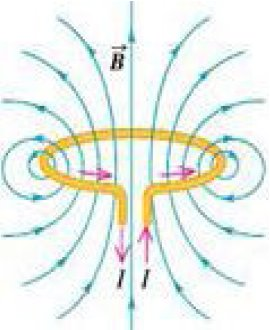
\includegraphics[width=0.48\textwidth]{images/inductive_ring.jpg}\label{fig:magnetic_field}
  \end{center}
  \vspace{-20pt}
  \caption{Το μαγνητικό πεδίο που δημιουργείται πάνω σε έναν αγώγιμο δακτύλιο καθώς σε αυτόν περνά εναλλασσόμενο ρεύμα.}
  \vspace{-10pt}
\end{wrapfigure}
Στην συνέχεια, αν ένας δεύτερος δακτύλιος έρθει κοντά στον πρώτο δακτύλιο τότε μπορεί να "πιάσει" κάποιο μέρος του μαγνητικού πεδίου το οποίο στην συνέχεια
δημιουργεί, επειδή είναι ταλαντούμενο το μαγνητικό πεδίο, ένα εναλλασσόμενο ρεύμα πάνω του. Το ρεύμα που δημιουργείται στο δεύτερο δακτύλιο μπορεί να χρησιμοποιηθεί
για να τροφοδοτήσει ηλεκτρικές συσκευές.  Αυτό το σύστημα μετάδοσης ενέργειας (ή καλύτερα μετατροπής της ενέργειας) χρησιμοποιείται εδώ και πάνω από έναν αιώνα στους
ηλεκτρικούς μετατροπείς και ηλεκτρικές γεννήτριες.

Για την ασύρματη μεταφορά ενέργειας χρησιμοποιείται η ίδια λογική μόνο που αντί για απλούς δακτύλιους, χρησιμοποιούνται πολύ υψηλής ποιότητας πηνία τα οποία
παρουσιάζουν επίσης πολύ υψηλό παράγοντα Q που τους επιτρέπει να μεγαλώσουν την απόσταση μεταξύ τους σε σχέση με την προηγούμενη περίπτωση. Για να μεγαλώσει η απόδοση
του συτήματος τα δύο πηνία θα πρέπει να είναι επίσης ισχυρά συνδεδεμένα (strongly coupled), δηλαδή ο συντελεστής αμοιβαίας επαγωγής να είναι κοντά στο 1\footnote{Ο
συντελεστής αμοιβαίας επαγωγής είναι πάντα μεταξύ του 0 και του 1 και εξαρτάται από την διάταξη των 2 πηνίων. Ουσιαστικά πρόκειται για το ποσοστό της μαγνητικής ροής
του πρώτου πηνίου/δακτύλιου κλπ "κόβει" το δεύτερο πηνίο/δακτύλιο κλπ. Μικρός συντελεστής σημαίνει οτι τα πηνία είναι ασθενά συνδεδεμένα και επομένως στο 2ο πηνίο
χάνεται το μεγαλύτερο μέρος της μαγνητικής ροής. Αντίθετα ισχυρά συνδεδεμένα σημαίνει οτι "κόβεται" μεγάλο μέρος της μαγνητικής ροής.}.

Η διαφορά με τις μέχρι τώρα προσπάθειες είναι οτι σε αυτό το μοντέλο προκειμένου να επιτευχθεί μεγαλύτερη απόδοση στην μεταφορά ενέργειας, θα πρέπει ο πομπός και ο
δέκτης έχουν και οι δύο την ίδια φυσική συχνότητα, δηλαδή τα 2 αυτά πηνεία θα πρέπει
να έχουν την ίδια ιδιοσυχνότητα (resonance)\footnote{Η ιδιότητα της ιδιοσυχνότητας υπάρχει σε πολλά διαφορετικά συστήματα. Μπορεί να θεωρηθεί  ως  η φυσική
συχνότητα στην οποία η ενέργεια μπορεί να προστεθεί με βέλτιστη απόδοση στο σύστημα. Ένα παράδειγμα είναι αυτό της κούνιας που κάνει ένα παιδί, το οποίο μπορεί να
θεωρηθεί ως μια ταλάντωση. Το παιδί μπορεί να κινείται μπρος-πίσω σε ρυθμό που καθορίζεται από το μήκος της κούνιας. Μπορεί να κάνει την κούνια να κινηθεί με
μεγαλύτερο μήκος αν συχρονίσει ταυτόχρονα τις κινήσεις των χεριών και των ποδιών του με την κίνηση της κούνιας. Ένα άλλο χαρακτηριστικό παράδειγμα της ιδιοσυχνότητα
είναι η θραύση ενός ποτηριού γεμάτο με κρασί από μία πολύ συγκεκριμένη νότα (συχνότητα) που τραγουδάει ένας τραγουδιστής.}. Ταυτόχρονα η απόστασή τους να μην
υπερβαίνει το $\frac{1}{4}$ του μήκους κύματος του πομπού, προκειμένου ο δέκτης να λαμβάνει αρκετό μαγνητικό πεδίο. Ένα παράδειγμα του συνολικού συστήματος φαίνεται
στην εικόνα \ref{fig:mit_exper0}.    


\begin{figure}[h]
	\centering
	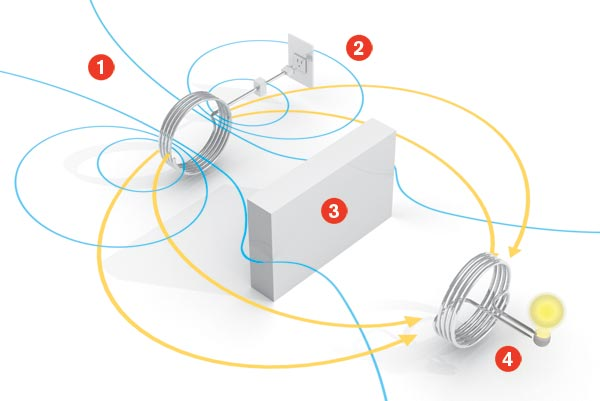
\includegraphics[width=0.9\textwidth]{images/mit_exper0.jpg}
	\caption{Ένα παράδειγμα της νέας τεχνολογίας ασύρματης μετάδοσης ενέργειας: (1) Πηνίο κατασκευασμένο από χαλκό με ιδιοσυχνοτητα.
    (2) Τροφοδοσία. (3) Εμπόδιο το οποίο προσπαρνάται χωρίς να υπάρχει απώλεια στην απόδοση. (4) Χάλκινο πηνίο με ίδια ιδιοσυχνότηα συνδεδεμένο με μια λάμπα.}
	\label{fig:mit_exper0}
\end{figure}


Οι ερευνητές του MIT επιτυχημένα παρουσίασαν στην πράξη αυτή την θεωρία. Χρησιμοποιώντας 2 χάλκινα πηνία με 5 γύρους, και διάμετρο 60 εκατοστά, τα οποία ήταν
τοποθετημένα σε απόσταση 2 μέτρων μεταξύ του, κατάφεραν να πετύχουν μεταφορά ενέργειας από το ένα πηνίο στο άλλο με απόδοση 45\% και τελικά τροφοδοτόντας μία λάμπα
60 Watt στο δεύτερο πηνίο. Τα πηνία ήταν σχεδιασμένα έτσι ώστε να έχουν ακριβώς την ίδια ιδιοσυχνότητα, στα 9,9MHz με μήκος κύματος τα 30 μέτρα και ήταν τοποθετημένα
ακριβώς στον ίδιο (κάθετο) άξονα. Φωτογραφίες από το πείραμα φαίνονται στην εικόνα \ref{fig:mit_eperiments}.
\begin{figure}[h]
  \centering
  \subfloat{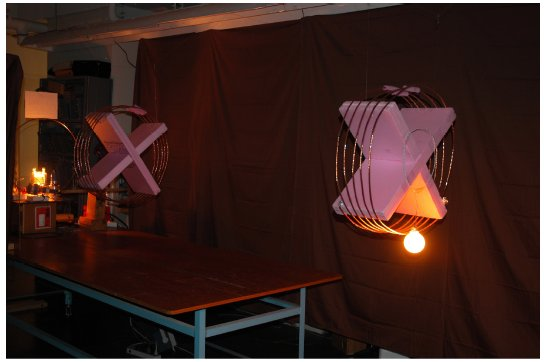
\includegraphics[width=0.48\textwidth]{images/mit_exper1.jpg}}
  \subfloat{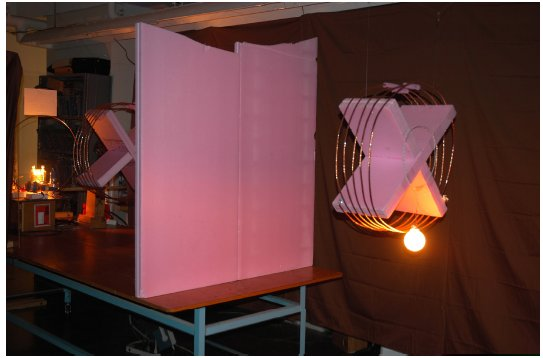
\includegraphics[width=0.48\textwidth]{images/mit_exper2.jpg}}
  \caption{Το πείραμα που έγινε στο mit είχε απόδοση κοντά στο 45\%.}
  \label{fig:mit_eperiments}
\end{figure}

Όπως φαίνεται και στις εικόνες, ακόμα και αν τοποθετούνταν ένα εμπόδιο ανάμεσα στα 2 πηνία, η λάμπα συνέχιζε να άναβε, δηλαδή η μεταφορά ενέργειας συνέχιζε να
υφίσταται με σχεδόν την ίδια απόδοση. Αυτό συνβαίνει λόγω της γεωμετρίας του μαγνητικού πεδίου που δημιουργείται.

Η τεχνολογία της ασύρματης μεταφοράς ενέργειας μπορεί άνετα να ενσωματωθεί στα ασύρματα δίκτυα αισθητήρων καθώς η λογική της είναι πολύ απλή. Ο κάθε κόμβος θα πρέπει
να έχει επιπλέον κυκλώματα με κύριο συστατικό το πηνίο το οποίο θα του επιτρέπει την φόρτισή του. Επίσης θα μπορεί να υπάρχει ένας κινητός κόμβος (robot) ο οποίος με
κατάλληλους αλγορίθμους θα κινείται στην περιοχή του δικτύου και θα φορτίζει τον κάθε κόμβο. Θα πρέπει όμως όλοι οι κόμβοι να έχουν συγκεκριμένη ιδιοσυχνότητα η
οποία θα είναι ίδια με την ιδιοσυχνότητα του πομπού, δηλαδή του κινητού κόμβου. Επίσης δεν θα είναι αναγκαίο ο κινητός κόμβος να έχει άμεση επαφή (<1 εκατοστού) με
τον στατικό κόμβο ανάλογα με το μήκος κύματος που θα χρησιμοποιείται ο κινητός κόμβος θα μπορεί να τον φορτίζει αποδοτικά και από πιο μακρινές αποστάσεις. Τέλος λόγω
των ιδιοτήτων της τεχνολογίας αυτής, ακόμα και αν υπάρχει ένα μικρό εμπόδιο το οποίο εμποδίζει την οπτική επαφή ανάμεσα στον κινητό κόμβο και τον στατικό κόμβο, η
μεταφορά ενέργειας μπορεί και πάλι να επιτευχθεί με την ίδια σχεδόν απόδοση. Ένα παράδειγμα ενός κινητού κόμβου που φορτίζει τους στατικούς κόμβους σε ένα ασύρματο
δίκτυο αισθητήρων με αυτή την τεχνολογία παρουσιάζεται στην εικόνα \ref{fig:wrsn_example}. Εφόσον η τεχνολογία αυτή μπορεί να ενσωματωθεί σε ΑΔΑ συστήματα, μένει να
κατασκευαστούν αλγόριθμοι και στρατηγικές φόρτισης προκειμένου να διαμοιράζεται η πολύτιμη ενέργεια του φορτιστή όσο πιο δίκαια γίνεται. Αυτό το πρόβλημα αναλύεται
στο επόμενο κεφάλαιο.


\begin{figure}[h]
	\centering
	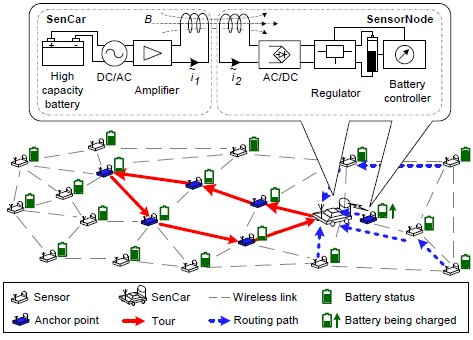
\includegraphics[width=0.6\textwidth]{images/sencar_example.jpg}
	\caption{Ένα παράδειγμα ενός ασύρματα επαναφορτιζόμενο δικτύου αισθητήρων (εξαγμένο από το \cite{yuanyuan_joint}).}
	\label{fig:wrsn_example}
\end{figure}
